\begin{table}[htbp]
  \centering
  \caption{PacBio sequencing statistics}
  \begin{tabular}{lccc}
  \hline
  & Hd-rR & HNI & HSOK \\ \hline
  Number of cells & 38 (P6-C4) + 35 (P5-C3) + 78 (P4-C2) & 24 (P5-C3) + 144 (P4-C2)	& 97 (P6-C4) \\
  Number of filtered subreads & 13,359,879	& 14,777,797 & 5,527,528 \\
  Total bases (bp) & 87,095,247,396 & 52,830,178,508 & 60,649,832,062 \\
  Average read length (bp) & 6,519 & 3,575 & 10,972 \\
  \hline
\end{tabular}

  \label{sequencing_stats}
\end{table}

\begin{table}[htbp]
  \centering
  \caption{Centromeric repeat genomic abundance}
  \begin{tabular}{p{1.5cm}p{2.5cm}p{3cm}p{3cm}p{3.5cm}p{2.5cm}}
  \hline
  strain & total subreads & passed subreads & passed subreads & repeats in passed subreads & estimated genomic abundance \\ \hline
  Hd-rR & 13,359,879 & 4,586,550 (34.33\%) & 34,933,754,979 bp & 354,930,731 bp (1.02\%) &  8.13 Mb \\
  HNI   & 14,777,797 & 7,265,969 (49.17\%) & 28,478,925,597 bp & 338,807,989 bp (1.19\%) &  9.52 Mb \\
  HSOK  &  5,527,528 & 1,955,979 (35.39\%) & 23,106,352,588 bp & 460,716,149 bp (1.99\%) & 15.95 Mb \\
  \hline
\end{tabular}

% \begin{tabulary}{18cm}{LRRRRR}
%   \hline
%   strain & total subreads & passed subreads & passed subreads & repeats in passed subreads & estimated genomic abundance \\ \hline
%   Hd-rR & 13,359,879 & 4,586,550 (34.33\%) & 34,933,754,979 bp & 354,930,731 bp (1.02\%) &  8.13 Mb \\
%   HNI   & 14,777,797 & 7,265,969 (49.17\%) & 28,478,925,597 bp & 338,807,989 bp (1.19\%) &  9.52 Mb \\
%   HSOK  &  5,527,528 & 1,955,979 (35.39\%) & 23,106,352,588 bp & 460,716,149 bp (1.99\%) & 15.95 Mb \\
%   \hline
% \end{tabulary}

  \label{centromeric_repeat_genomic_abundance}
\end{table}

%% FISH
\begin{figure}[p]
  \centering
  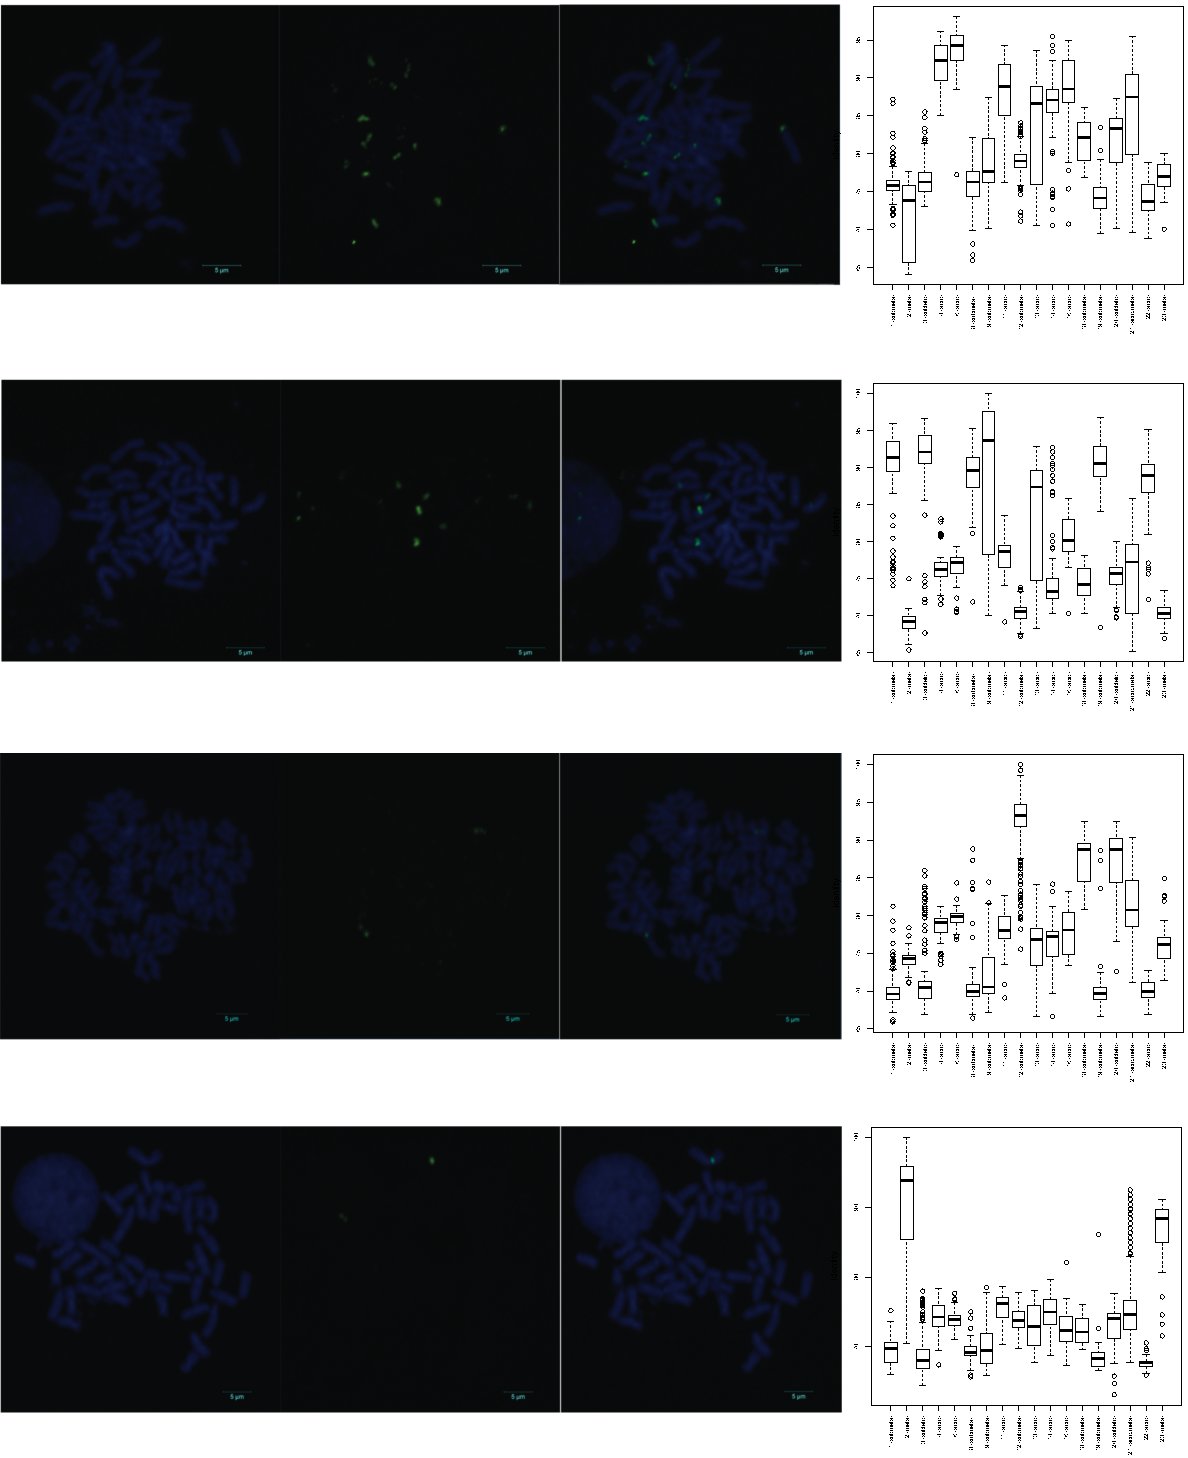
\includegraphics[width=\linewidth]{fish_each_probes.pdf}
  \caption{
    FISH with four probes. (Left) FISH; DNA is stained with DAPI (left); probes are stained green (center); combined (right). (Right) similarity of the probe sequence to satellite sequences in each chromosomes are plotted \textit{in silico}. The top probe used the candidate centromeric satellite sequence identified by Melters \textit{et al.} \cite{Melters2013} and hybridized to 5$\sim$7 pairs of chromosomes. The other probes were additionally designed and hybridized to other $\sim$6, 1 and 1 pairs of chromosomes, respectively.
  }
  \label{fish_each}
\end{figure}


%% Centromeric repeat distribution
\begin{figure}[p]
  \centering
  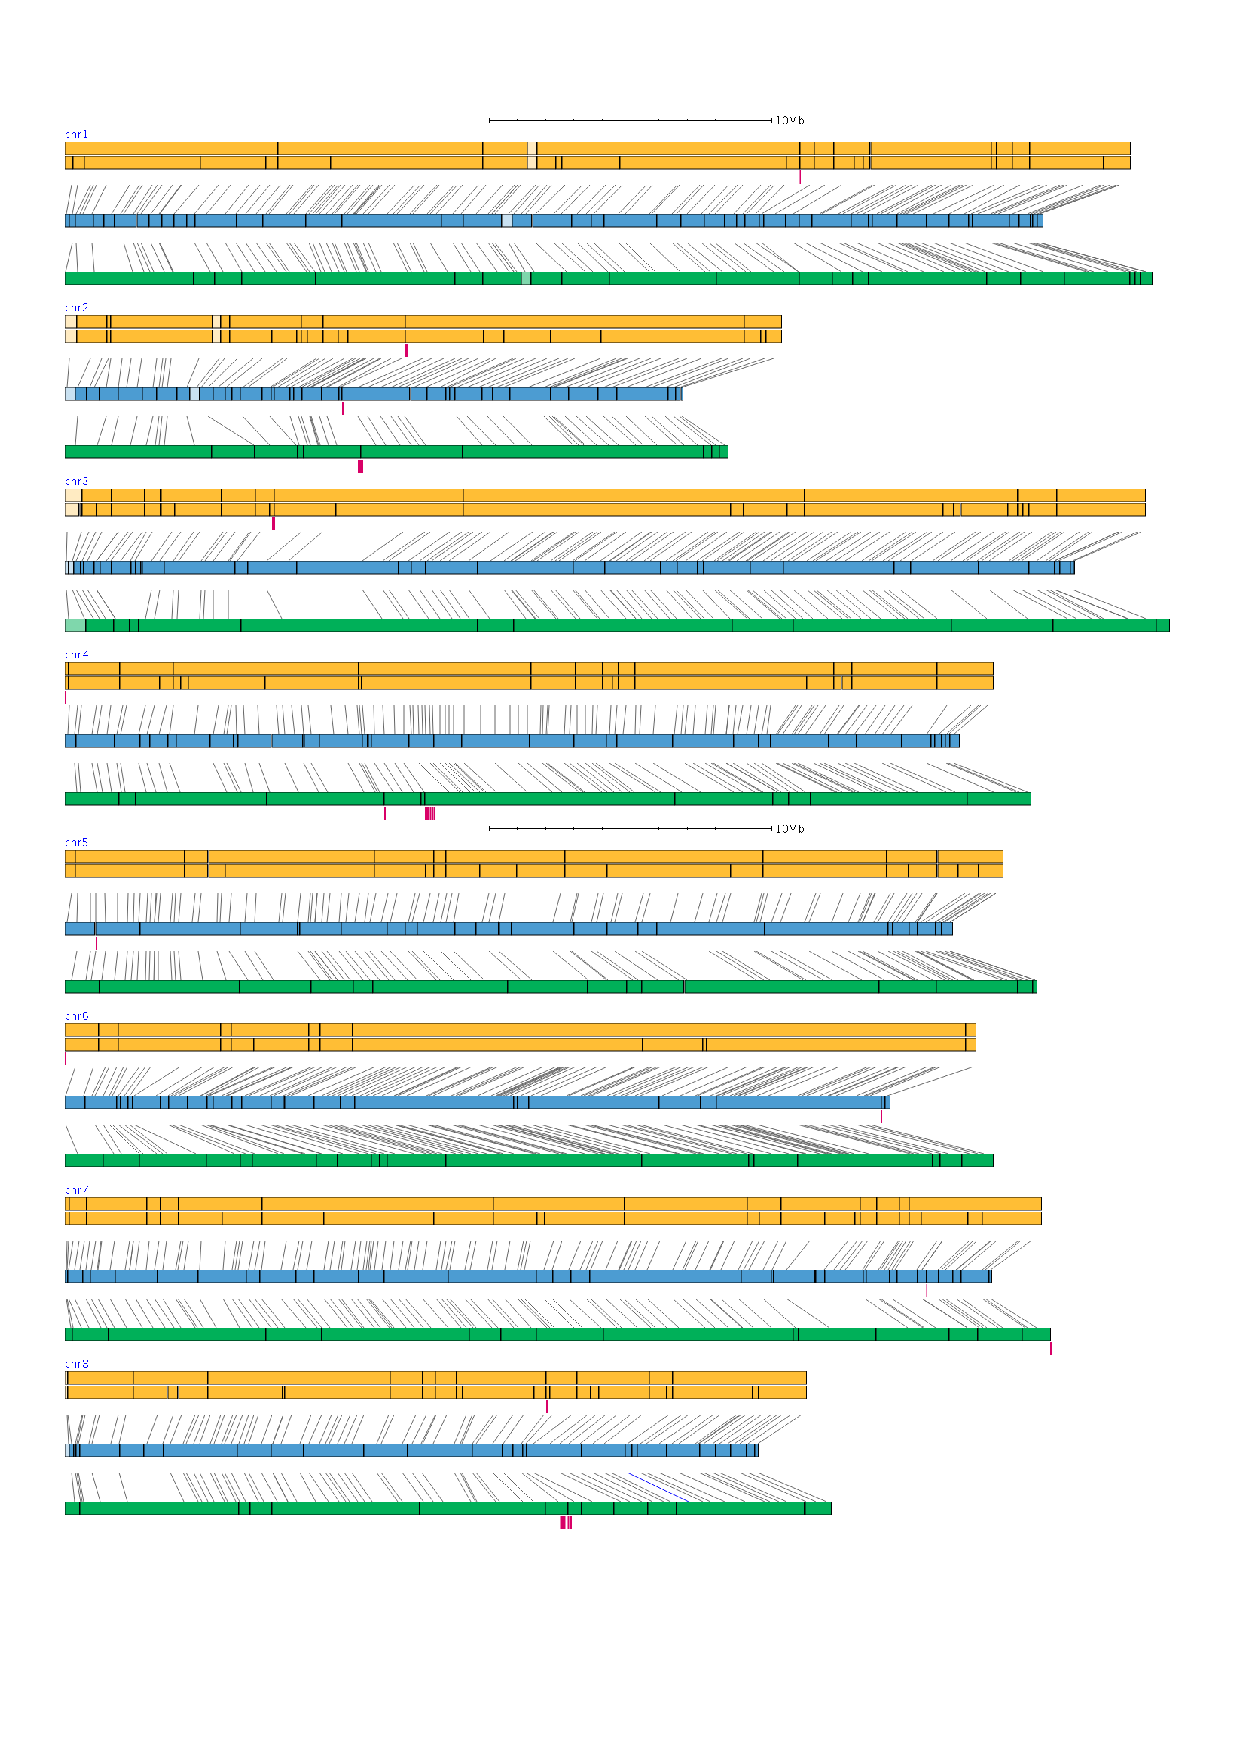
\includegraphics[width=\linewidth]{repeat_distribution_1.pdf}
  \caption{
    Centromeric repeat distribution. Yellow, Hd-rR scaffolds (upper) and contigs (lower); blue, HNI contigs; green, HSOK contigs; red, centromeric repeats; grey, corresponding genetic markers.
  }
  \label{fig:repeat_distribution}
\end{figure}

\addtocounter{figure}{-1}
\begin{figure}[p]
  \centering
  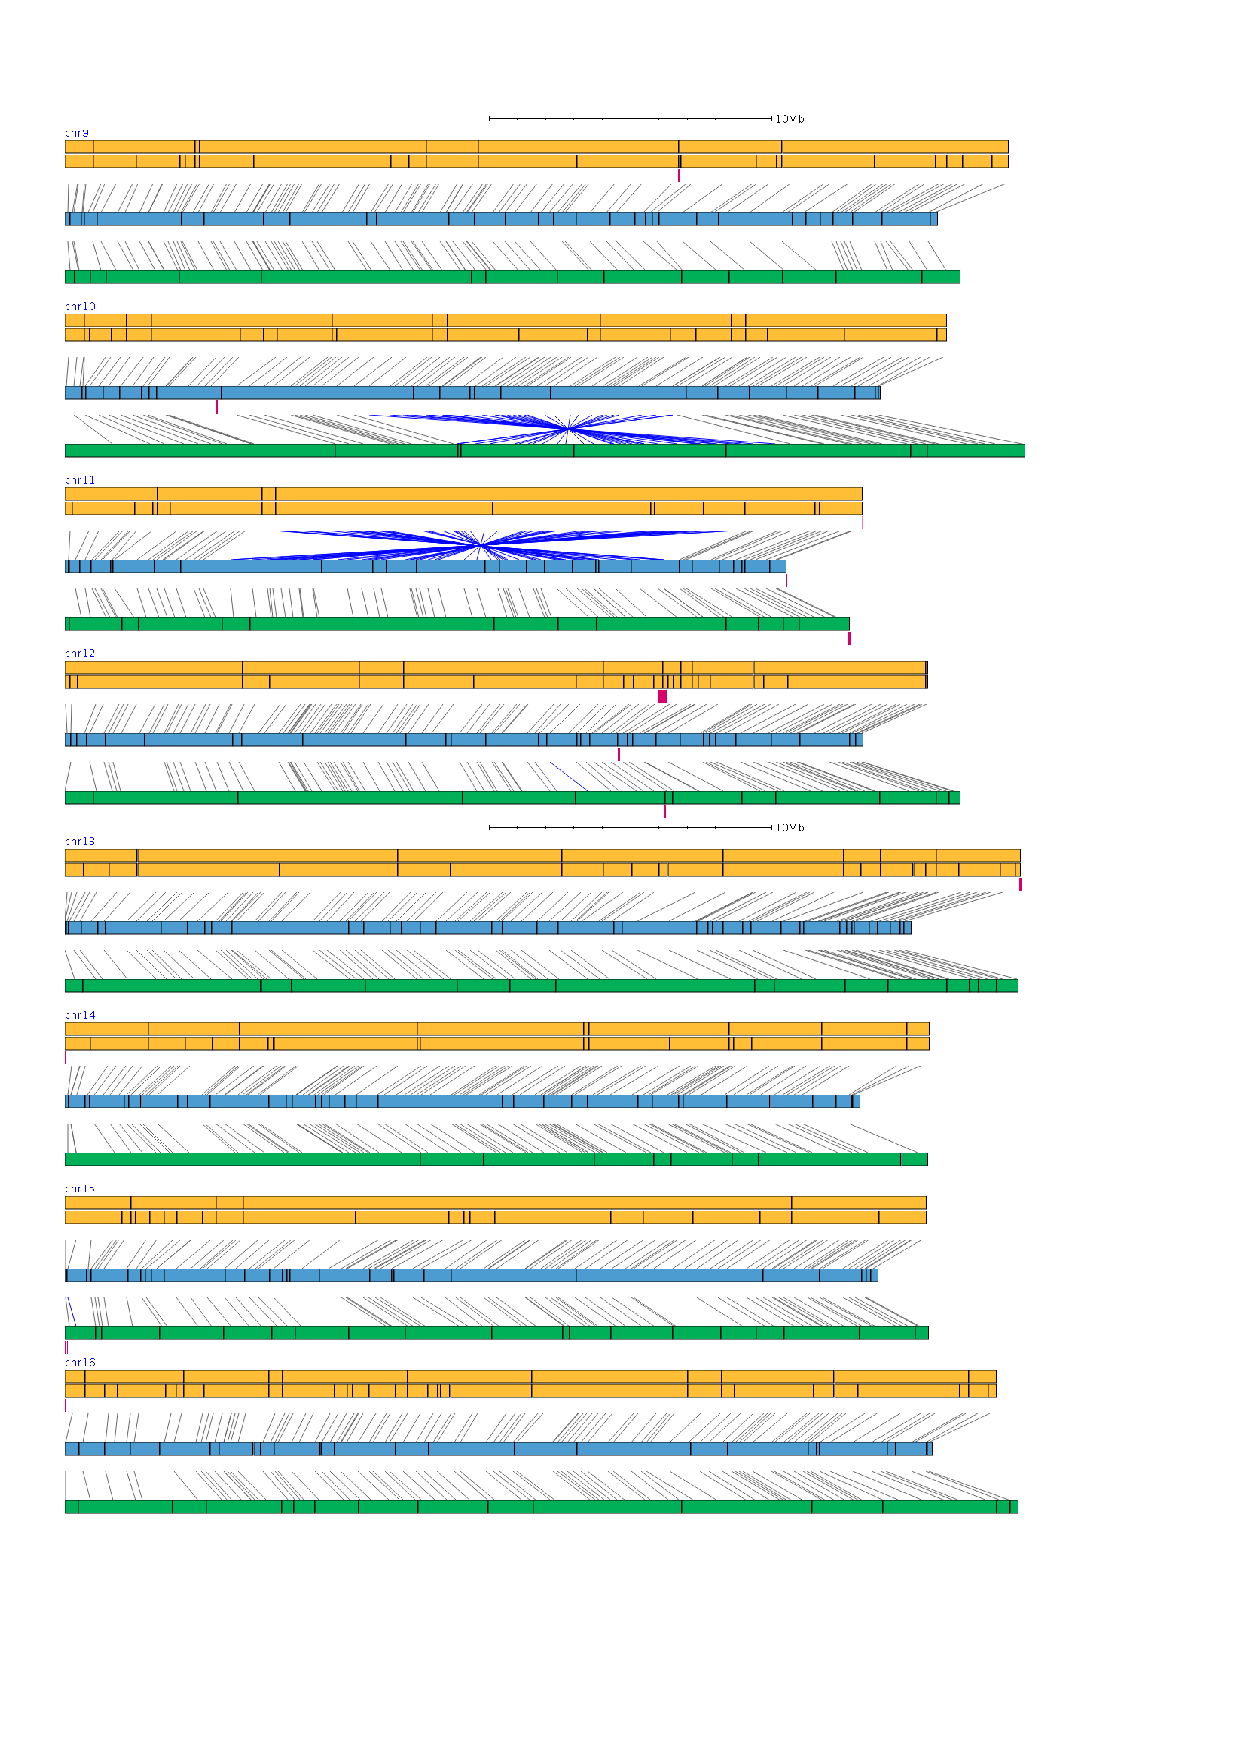
\includegraphics[width=\linewidth]{repeat_distribution_2.pdf}
  \caption{
    Centromeric repeat distribution. Yellow, Hd-rR scaffolds (upper) and contigs (lower); blue, HNI contigs; green, HSOK contigs; red, centromeric repeats; grey, corresponding genetic markers.
  }
  \label{fig:repeat_distribution}
\end{figure}

\addtocounter{figure}{-1}
\begin{figure}[p]
  \centering
  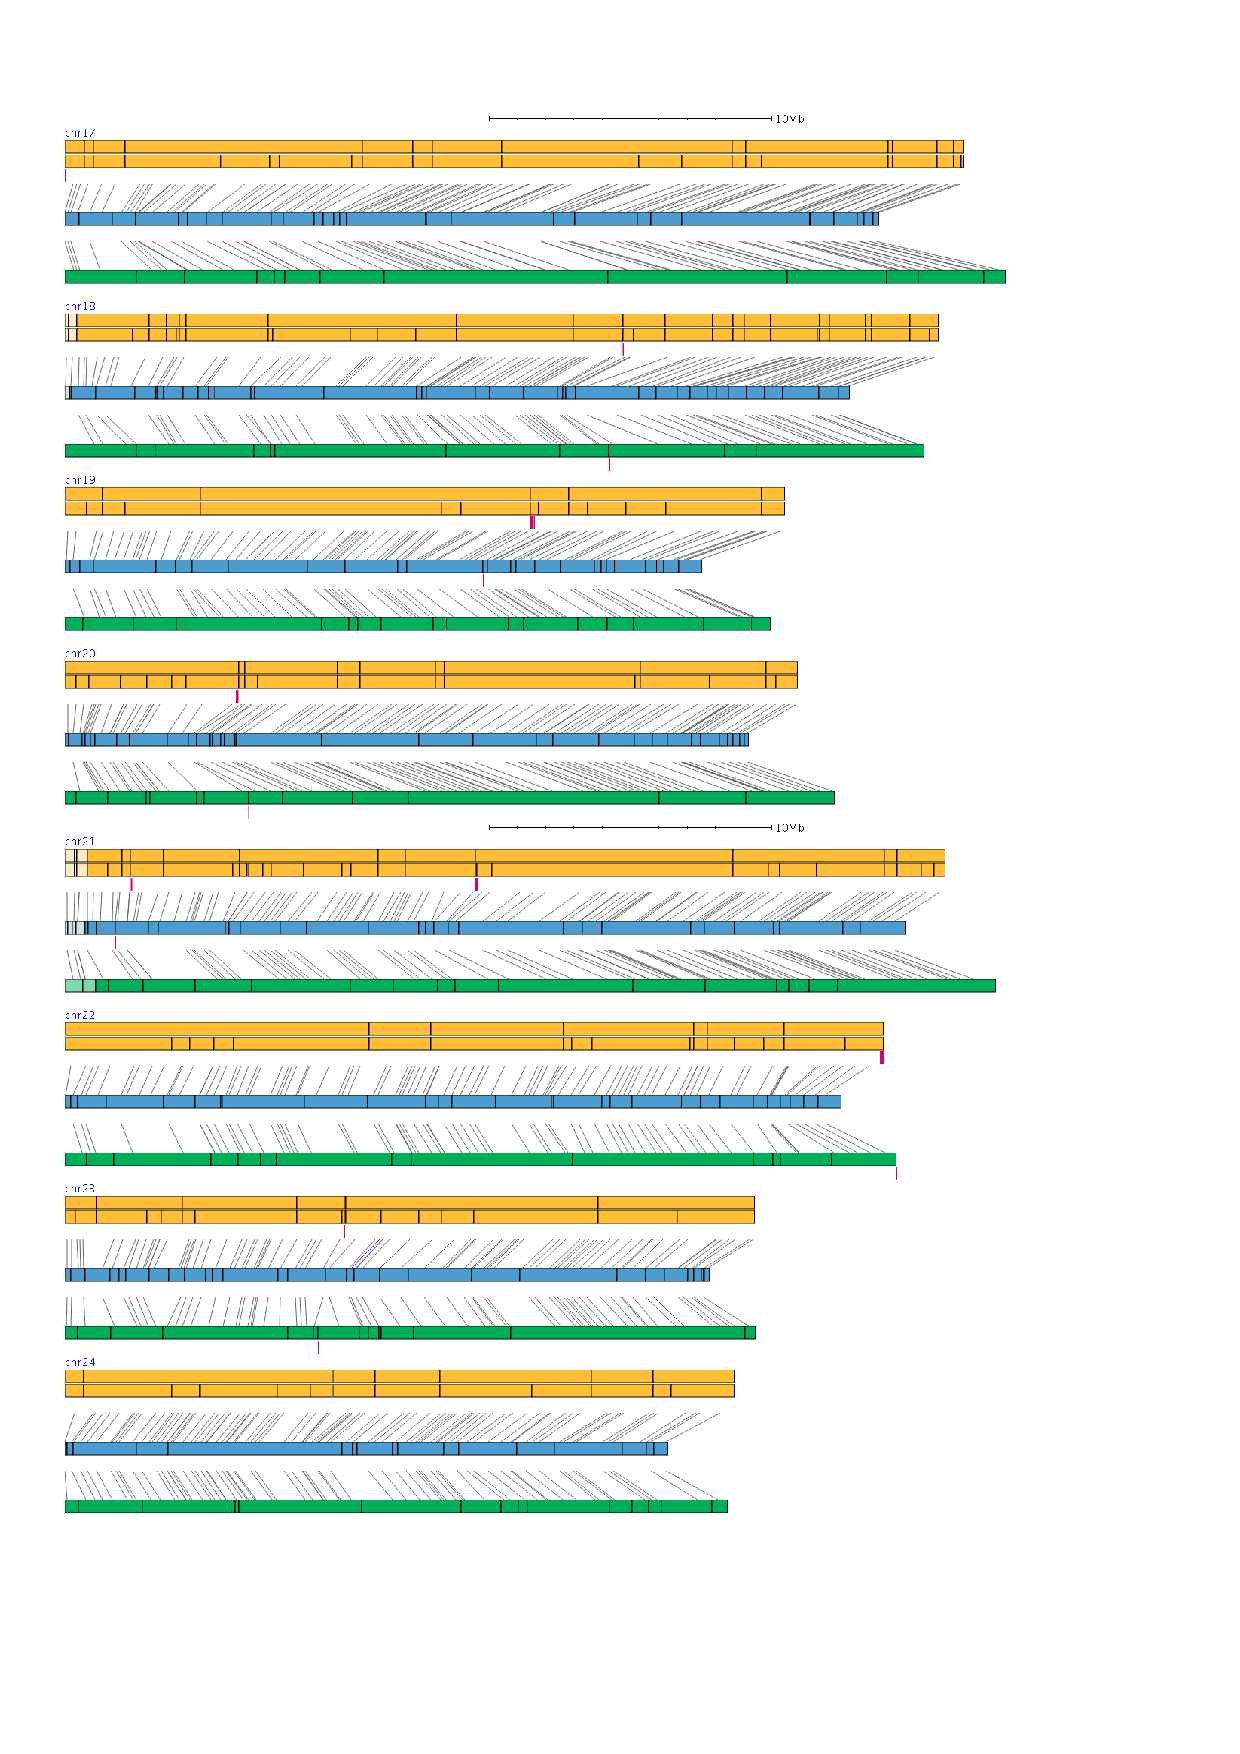
\includegraphics[width=\linewidth]{repeat_distribution_3.pdf}
  \caption{
    Centromeric repeat distribution. Yellow, Hd-rR scaffolds (upper) and contigs (lower); blue, HNI contigs; green, HSOK contigs; red, centromeric repeats; grey, corresponding genetic markers.
  }
  \label{fig:repeat_distribution}
\end{figure}



\begin{figure}[p]
  \centering
  %\includegraphics{}
  \caption{
    Centromere landscapes in the medaka genomes
  }
  \label{centromere_landscape}
\end{figure}

\begin{figure}[p]
  \centering
  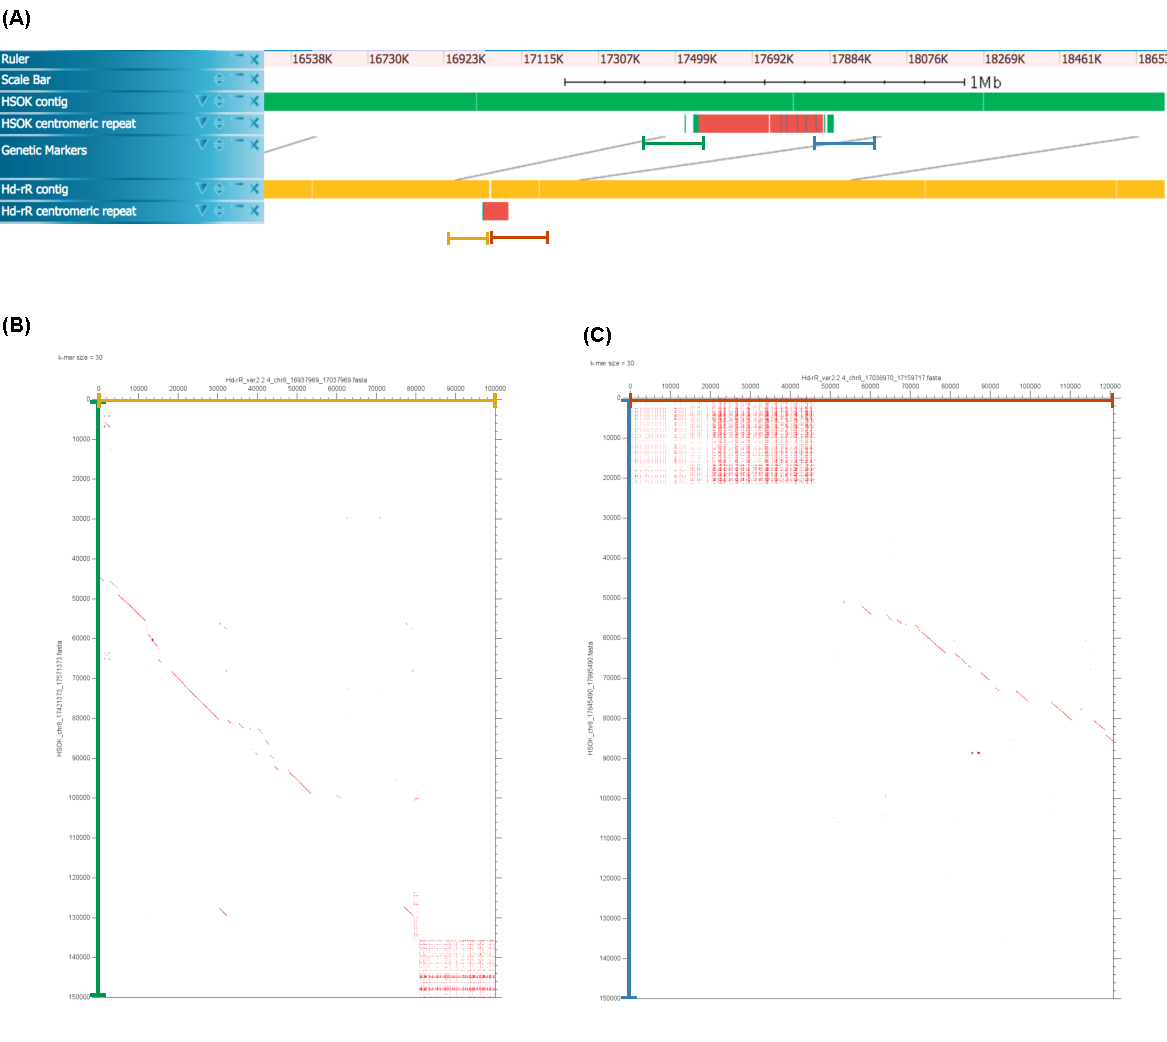
\includegraphics[width=\linewidth]{chr8_transition.pdf}
  \caption{
    (A, B, C) Comparison of the centromeric transitional regions of chromosome 8 of Hd-rR and HSOK.
  }
  \label{other_chroms_transition}
\end{figure}

\addtocounter{figure}{-1}
\begin{figure}[p]
  \centering
  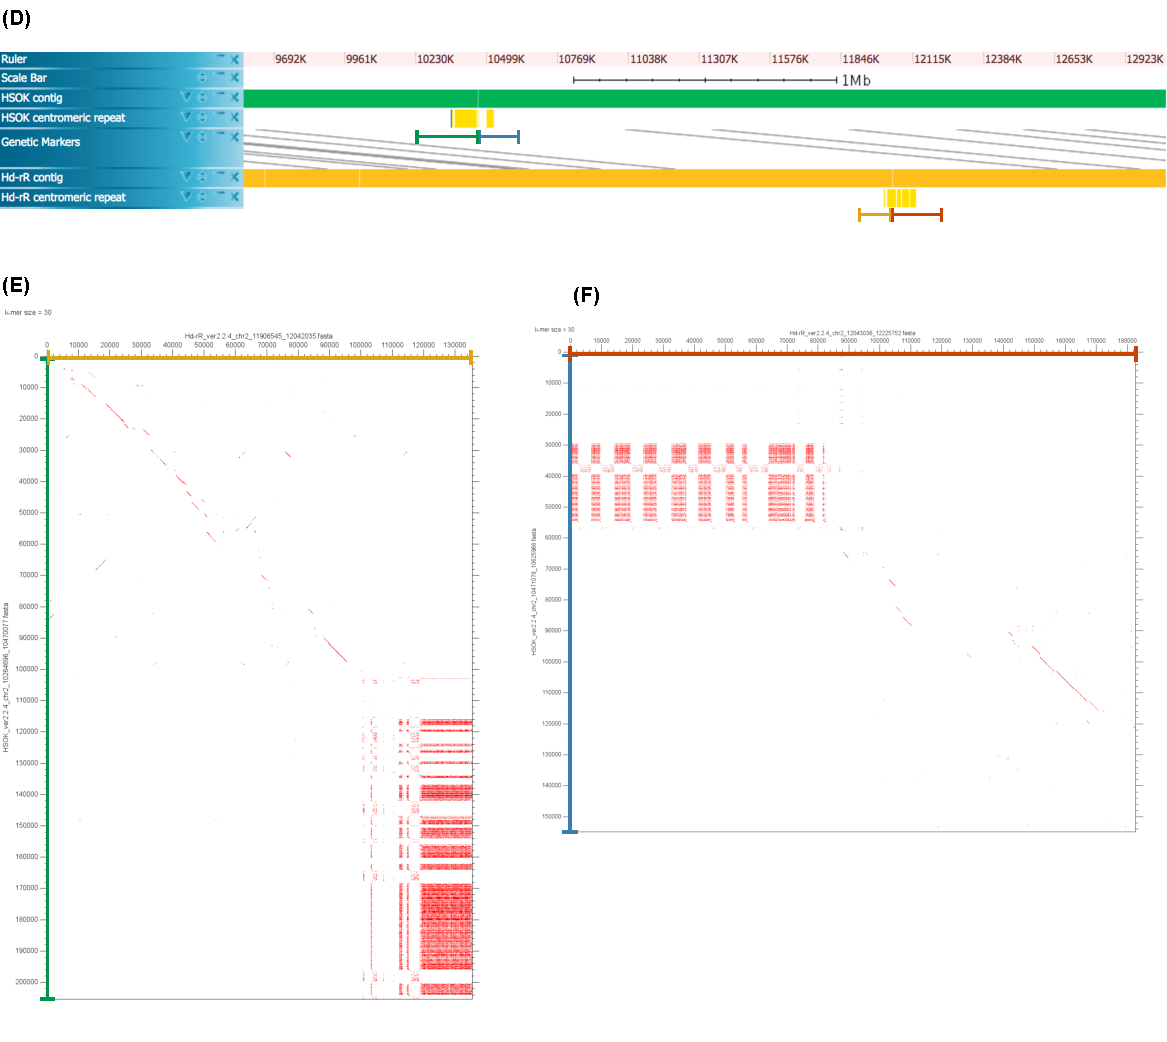
\includegraphics[width=\linewidth]{chr2_transition.pdf}
  \caption{
    (D, E, F) Comparison of the centromeric transitional regions of chromosome 2 of Hd-rR and HSOK.
  }
\end{figure}
